First we will plot these lines which are the constraints and the area enclosed by is the region we are interested in.

\begin{figure}[h]
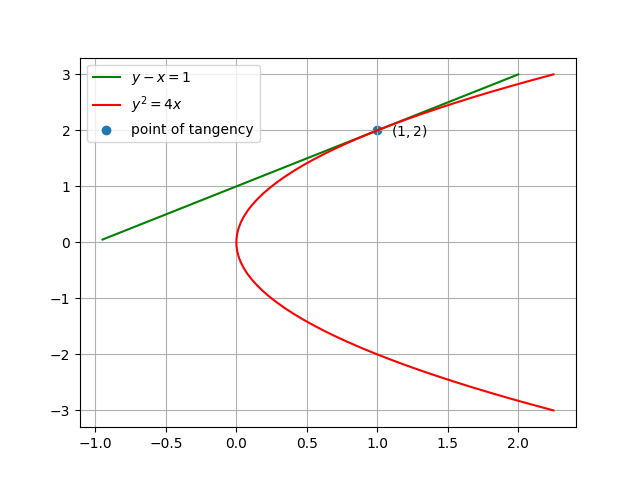
\includegraphics[width=\columnwidth]{./solutions/5/1/9/figs/Figure_1.png}
\caption{optimal point through the intersection of various lines}
\label{eq:solutions/5/1/9/fig:Figure_1}
\end{figure}

The four points are the points which will maximize and minimize the function.These corner points are :
\begin{align*}
    A=(60,30)
\\
    B=(40,20)
\\
    C=(60,0)
\\
    D=(120,0)
\end{align*}

Value of Z at point

\begin{align*}
     A= 5\times 60 + 10 \times 30 =600
\\
     B= 5\times 40 + 10 \times 20 =400
\\
     C= 5\times 60 + 10 \times 0 =300
\\
     D= 5\times 120 + 10 \times 0 =600
\end{align*}

We can see that our function Z is maximum at points A and D that is (60,30) and (120,0)\\
and\\
Z is minimum at point C that is (60,0)\\
The given problem can be expressed in general as matrix inequality as:
\begin{align}
\max_{\vec{x}} Z &= \myvec{5 & 10}\vec{x}
\\
s.t. \quad 
\myvec{
1 & 2
\\
-1 & -1
\\
-1 & 2
}
\vec{x} &\preceq \myvec{120\\-60\\0}
\\
\vec{x} &\succeq \vec{0}\\
\vec{y} &\succeq \vec{0}
\end{align}
\begin{align}
\max_{\vec{x}} &\vec{c}^{T}\vec{x}
\\
s.t. \quad \vec{A}\vec{x} &\le \vec{b},
\\
\vec{x} &\succeq\vec{0}\\
\vec{y} &\succeq \vec{0}
\end{align}
%
where
\begin{align}
\vec{c} &= \myvec{5 \\ 10}
\\
\vec{A} &=
\myvec{
1 & 2
\\
-1 & -1
\\
-1 & 2
}
\\
\vec{b}&=\myvec{120\\-60\\0}
%
\end{align}
%
%
